
\subsection{Introduction}

Ce chapitre présente l'étude existante avec son ensemble d'approches pour une exécution fiable des services Web composites.
Cet étude consiste l'exécution auto-corrective (self-healing) d'une manière dynamique et automatique, elle vise le même objectif de ce mémoire mais les méthodologie changent. 

L'ensemble des approches proposés peuvent être présenter sous forme de trois principaux partis.
Dans un premier temps on va voir une approche pour l'exécution tolérante aux pannes des services Web composite basée sur la récupération en avant et en arrière, et définie par le formalisme de réseaux de Petri Colorés, ensuite sur le même formalisme la deuxième approche consiste la proposition d'un mécanisme de point de contrôle, et finalement après une étude sur l'impact des différentes stratégies de récupération sur les services Web composite, la troisième approche apporte un modèle de décision dynamique de la stratégie de récupération en terme d'impact sur la qualité de service pour la tolérance aux pannes de services Web composites.


\subsection{Récupération des CWS Réseaux de Petri Colorés}

En utilisant les réseaux de Petri Colorés les auteurs ont formalisé les services Web composites, leur exécution, et leurs stratégies de tolérance aux pannes, et il ont proposé un framework pour une exécution distribuée fiable et tolérante aux pannes pour les services Web Composites.

Le framework est composé de deux types de composants \cite{1} : 

- Un Coordinateur d'Agents : Composant responsable de la gestion des aspects globaux d'exécution des services Web composites.

- Agents de Service : ils exécutent les services et sont en charge du contrôle de l'exécution et de la tolérance au pannes.

Cette approche fournis les mécanismes de récupération en arrière par compensation, en avant par re-exécution de service et remplacement, la réplication, et le checkpointing, et assure une exécution tolérante aux pannes basé sur un modèle d'exécution distribué.

L'exécution des services Web composite peut être \cite{3} : 

- Séquentiel : Les services se basent sur les résultat des services précédents, et ne peuvent être invoqués tant que les services précédent ne sont pas terminés.

- Parallèle : Les services peuvent être invoqués d'une manière simultanée, car il n'y a pas des dépendances de flux de données entre eux.

Ces deux scénarios d'exécution ont un effet sur la propriété transactionnelle globale du service Web composite, pour cela il faut suivre le flux d'exécution défini par le graphe du service composite pour s'assurer que l'exécution séquentielle et parallèle satisfont la propriété transactionnelle globale.

\subsubsection{Architecture du Framework}

Les chercheurs ont proposé un Framework dont l'exécution du service composite est gérée par un Coordinateur d'Agents et une collection d'Agents de services, organisés dans architecture trois tiers.

\begin{figure}[H]
\begin{center}
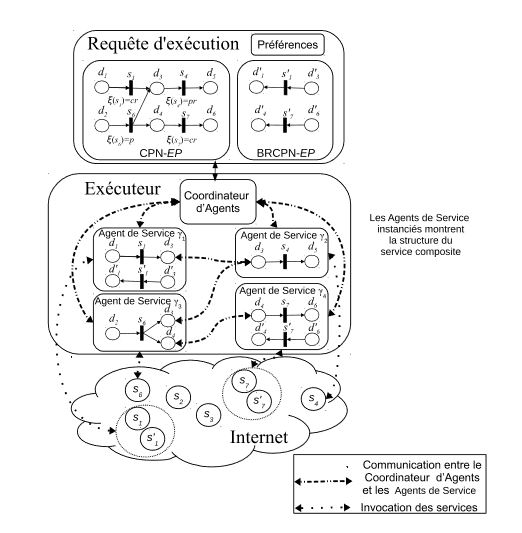
\includegraphics[width=1\linewidth]{images/architecture Frmwork.jpg}
\end{center}
\caption{Architecture d'exécution \cite{1}}
\label{fig:4}
\end{figure}


L’architecture du Framework est composée de trois niveaux principaux:

Le premier niveau : Le coordinateur d’agents reçoit le service composite et son graphe de compensation correspondant, qui sont représentés sous forme des réseau de Pétri Colorés, qui peuvent être générés d'une manière automatique ou manuelle.
Dans ce niveau le Coordinateur reçoit aussi une propriété qui lui indique si le mécanisme de checkpointing est activé ou non.

Le deuxième niveau: Le coordinateur d'Agents lance un Agent de Service pour chaque service composant du service Web composite, chaque agent de service sera responsable du contrôle de l'exécution de son service, ses rôles sont les suivants \cite{1}:

    - Responsabilité de l'invocation de services ;

    - Surveillance de l'exécution des services correspondants ;
    
    - Envoi des résultat selon le flux d'exécution ;
    
    - Lancement des stratégies de tolérance aux pannes en cas de panne.

Le troisième niveau : consiste l'interaction des agents de services avec l'ensemble des services correspondants.

L'objectif de cet architecture est de répartir la responsabilité de l'exécution d'un service Web composite à travers de plusieurs agents de service, pour que le modèle logique de l'exécuteur proposé permet une exécution distribuée et une indépendance de la mise en oeuvre 

\subsection{Modélisation des stratégies de récupération basées sur QoS}

Après les évolutions des recherches, les auteurs ont découvert a travers leur étude qu'il y a des impacts des différentes stratégies de récupération sur les services Web composite et plus précisément sur sa qualité de service (QoS). C'est pour cela ils ont décidé de proposer une approche pour une décision dynamique des stratégies de récupération.

Pour fournir un choix dynamique de la stratégie de tolérance aux pannes, les auteurs ont proposé une approche auto-corrective (Self-Healing) pour les services Web composites.
Dans l'auto-correctif les agents de services sont des agents basés sur des connaissances, c'est à dire ils sont basés sur l'ensemble des information qu'ils ont sur le service Web composite, sur eux mêmes, et sur ce qui est attendu et ce qu'il se passe réellement pendant l'exécution, pour qu'ils puissent finalement faire la sélection de la stratégie de tolérance aux pannes.

Indépendamment de la technique utilisée pour l'estimation des critères de Qualité de service,ils ont proposé que chaque service Web est annoté avec son temps d'exécution estimé, son prix, sa réputation et sa propriété transactionnelle. Grâce aux critères des services composants, il est possible de calculer la Qualité de service d'un service Web composite en calculant des différents critères.

Sur cette base, la conception sera sous forme d'une boucle d'auto-guérison/auto-correction par agent de service pour effectuer la détection, le diagnostic et la récupération d'une manière décentralisée \cite{1}.


\begin{figure}[H]
\begin{center}
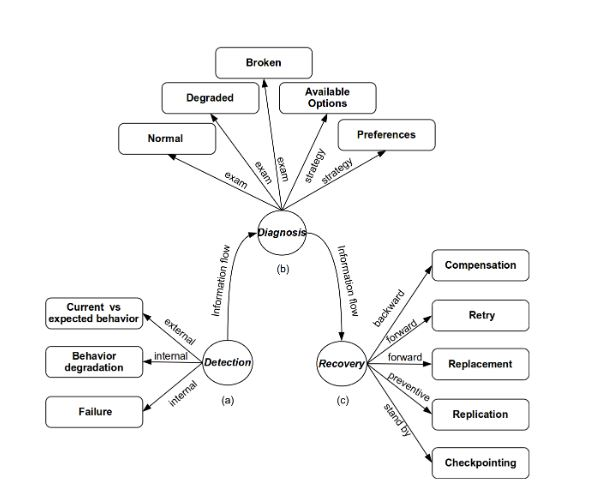
\includegraphics[width=1\linewidth]{images/Boucle auto-corrective des Agents de Service.jpg}
\end{center}
\caption{Architecture d'exécution \cite{1}}
\label{fig:5}
\end{figure}

- Le composant detection : Dans ce composant, trois sources sont prises en compte une externe et deux internes. 
La source externe consiste l'information sur la Qualité de service attendu, par exemple, le cas où l'utilisateur peut permettre une certaine dégradation de la Qos.
La source interne concerne la dégradation de la Qualité de service des services composants (par exemple, les variations négatives dans le temps d'exécution et le prix), et concerne aussi les pannes de services.

- Le composant diagnosis : ce composant a le rôle d'analyse du problème et la détermination de l'état du service.
Il existe trois diagnostics possibles qui correspondent au trois états d'un système auto-correctif : normal ; degraded ; et broken. Le choix de la stratégie de récupération est influencé par les options disponibles ( par exemple, les propriétés transactionnelles, les services de remplacement disponible, etc.), et influencé aussi par les préférences de l'utilisateur (la QoS attendu, le checkpointing, etc).

- Le composant recovery :  Ce composant prend en charge l'exécution des mécanismes de tolérance aux pannes sélectionnés : la récupération vers l'arrière avec la compensation ; la récupération en avant par la reexécution ou remplacement ; la prévention grâce à la réplication ; ou le retardement d'exécution par le checkpointing.



\subsection{Évaluation expérimentale }

Les chercheurs ont mis leur approche en évaluation expérimentale, et ça par la mise en oeuvre du Framework  en utilisant un cas d'étude qui consiste un sénario et un environnement.
L'observation du cas d'étude a été sur trois systèmes différent :

Système sans tolérance au pannes : c'est un système qui n'a aucun mécanisme de tolérance aux pannes. et dans le cas ou un des services composants tombe en panne, une exception sera générée et l'exécution sera terminé.

Système transactionnel : c'est un système qui se base sur les propriétés transactionnelles des services composants pour prendre les décisions de récupération.

Système auto-correctif :  c'est un système qui se base sur l'ensemble d'information et règle contenu dans les bases de connaissances des agents de services.


Les résultat de l'évaluation expérimentale ont montré : l'importance et la nécessité d'avoir des mécanisme de tolérance aux pannes pour les services Web composite, ainsi que la manière avec laquelle les deux approches des propriétés transactionnelles et l'auto-corrective gèrent les pannes et prennent la décision de récupération.
L'évaluation expérimentale faite pendant cette étude suggère que la combinaison des propriétés transactionnelles avec des capacités d'auto-corrective permet de donner une intelligence aux systèmes d'exécution pour gérer les exigences de haut niveau pour les exécutions de services Web composites avec une intervention humaine minimale\cite{1}.

\subsection{Conclusion}

